\chapter{Determining the Curie Temperature of Kanthal-D wire}

Date: 15/11/2020

\section{Aim}

The magnetic properties of materials depend upon the atomic and molecular arrangements within the material. These alignments also depend upon the temperature of the material. 
The aim of this experiment is to understand how temperature affects the magnetic properties of the Kanthal-D wire.


\section{Background Theory}

Both naturally-occurring and human-made materials have a range of magnetic properties. \textit{Ferromagnetic } materials posses an intrinsic magnetic field. Materials which acquire a magnetic field in the presence of external magnetic fields are called \textit{para-magnetic} materials. \textit{Diamagnetic} materials are those which are not affected by external magnetic fields. \\
The origin of magnetism in materials lies in the motion and configuration of electrons within an atom. These electrons constitute a current and hence produce a tiny magnetic for each atom. Each atom is called to make a magnetic dipole. The arrangement and orientation of these elementary dipoles determine the overall magnetic properties. If these magnetic dipoles are naturally aligned and kept in that configuration by the inter molecular forces, then the magnetic fields enforce each other and, as a result, the material gets an overall intrinsic magnetic field. These materials are called ferromagnetic materials.\\
Combinations of atoms are called \textit{magnetic domains}. Atoms within these magnetic domains are aligned in a certain direction on average. If these domains are randomly distributed it cancels the overall magnetic field of the material. In some materials, atoms in the domains, and thus the domain itself,can be made to align if an external magnetic field is applied. \\
In ferromagnets atoms in domains are aligned in a certain preferred direction and held in that place with the inter-molecular forces . In figure 1, boundaries between randomly aligned domains is shown in the absence and presence of a external magnetic fields.
\begin{figure}[h!]
    \centering
    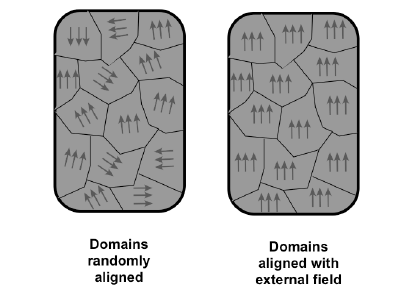
\includegraphics[width=\textwidth]{figures/Domains.png}
    \caption{Graph of y vs x}
    \label{fig:yx}
\end{figure}\\
The thermal energy of atoms and molecules tends to the disturb the alignment of elementary magnets. As the temperature increases, the alignment is disturbed, and above a critical temperature, the \textit{Curie temperature } $T_C$, a ferromagnetic turns into a para-magnet. \\
The electrical energy supplied in $\Delta t$ time supplied by voltage $V$ and current $I$ can be calculated by the following equation 
\begin{equation}
    E_E = V I \Delta t    
\end{equation}
The energy $E_a$, absorbed in raising the temperature of the Kanthal wire is given in terms of specific heat of Kanthal wire and change in temperature,
\begin{equation}
    E_a = mc(T_C - T_0)
\end{equation}
The energy radiated $E_r$ ratiated from the wire is,
\begin{equation}
    E_r = \epsilon \sigma S ({T_c}^4 - {T_0}^4)\Delta t
\end{equation}
Combining equation 1 and 2, and re-arranging the terms gives us the following equation.
\begin{equation}
    -(mcT_o + \epsilon \sigma S {T_0}^4 \Delta t + V I \Delta t) + m c T_C + \epsilon\sigma S {T_C}^4 \Delta t = 0
\end{equation}

\section{Description of Setup}
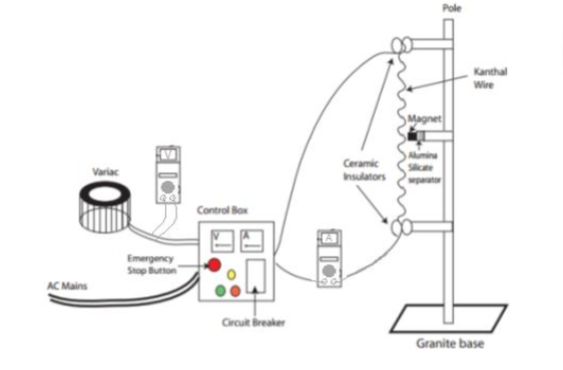
\includegraphics[width=10cm, height=7cm]{figures/fig9exp.png} \\
The experiment is set up as above where the variac is attached to an ammeter, voltmeter and a control box. The kanthal-D wire is attached to a magnet with minimum area contact on a pole. A stopwatch is used to record the time taken to reach curie temperature. A digital ammeter and voltmeter is used to get accurate readings since the control box isn't precise. 


\section{Method / Procedure}
The kanthal-D wire is attached to the magnet in such a way that there is minimum area in contact. The control box is set up and green button is pressed to turn it on. The output voltage is set on 25.3 V on a variac and the current is measured using a digital ammeter. To turn off the control box the toggle switch is pressed. After the wire is cooled, we turn on the toggle switch and start the stopwatch. When the wire snaps away from the magnet, the stopwatch is stopped and we turn off the toggle switch. The time is recorded and the heating element is cooled. Four more readings at the same voltage are taken. The same procedure is repeated for nine different voltages on variac with 5 readings at every voltage.  

\section{Data}

The mass m of the Kanthal wire is $2.35 \pm 0.01$ gm,diameter is  $0.723\pm 0.002$ mm , length is $100 \pm 0.1 $cm, c specific heat capacity (c) is $460 J {Kg}^{-1}{K}^{-1}$ and the Emissivity ($\epsilon $) is 0.7 . $T_0$ the room temperature is taken as $25^\circ$ C.\\
The following data was recorded 
\begin{center}
\begin{tabular}{|c|c|c|c|}
\hline
\textbf{s.No} & \textbf{Voltage (V)} & \textbf{Current (A)} & \textbf{Avg\_t(s)} \\ \hline
1             & 25.3                 & 5.63                 & 14.29              \\ \hline
2             & 26.3                 & 5.87                 & 9.09               \\ \hline
3             & 27.2                 & 6.04                 & 8.76               \\ \hline
4             & 28.8                 & 6.39                 & 6.84               \\ \hline
5             & 29.3                 & 6.57                 & 5.74               \\ \hline
6             & 31.5                 & 6.95                 & 4.98               \\ \hline
7             & 33.2                 & 7.31                 & 4.20               \\ \hline
\end{tabular}
\end{center}

\section{Data Analysis}

Solving the the degree 4 polynomial equation gives us the value of the Curie Temperature $T_C$ for value of Voltage and Current.  
\begin{center}
\begin{tabular}{|c|l|}
\hline
\textbf{s.No} & Curie Temperature (Tc) / K \\ \hline
1             & 999.595                     \\ \hline
2             & 959.303                     \\ \hline
3             & 974.734                     \\ \hline
4             & 967.115                     \\ \hline
5             & 943.795                     \\ \hline
6             & 958.587                     \\ \hline
7             & 953.408                     \\ \hline
\end{tabular}
\end{center}
The average value of the Curie Temperature $T_C$ is $692.220^\circ C$. The type A uncertainty in the value of the Curie Temperature is $6.820^\circ C$. The final value is $ 692.220 \pm 6.820 ^\circ C$

\section{Discussion \& Conclusion}

The expected value of the Curie Temperature for the Kanthal-D wire is $600 ^\circ $ C whereas the calculated value is $692.220^\circ C$. One of the reasons for this huge difference is the environmental losses. The long wire radiates more heat since the room is open and room temperature is not maintained. Furthermore, the time that is being recorded is very small and since its being recorded by a stopwatch there is human reaction time. Instead of using a stopwatch, record the motion by a video camera and then playback frame by frame to know the exact moment the wire becomes detached. The experiment should be carried out in a close environment. 



\section{MATLAB Script}
\lstinputlisting{matlabCodes/Experiment9.m}



